\documentclass[12pt]{article}
\usepackage[utf8]{inputenc}
\usepackage[T5]{fontenc}
\usepackage{graphicx,a4wide,framed,amssymb}
\usepackage{tikz}
\usetikzlibrary{decorations,decorations.pathmorphing,shadows}

\newcommand{\source}[1]{\begin{flushright}\emph{[#1]}\end{flushright}}

\newcommand{\MakeScribeTop}[1]{
\noindent
\begin{framed}
\noindent
 Algorithmique Avancée 2019
 \hfill
 École Centrale-Supélec
 \\[1em]
 \centerline{ \Large
#1
 }
 \\[1em]
\centerline{  \it Christoph Dürr, Nguyễn Kim Thắng}
\end{framed}
}



\begin{document}
    \MakeScribeTop{PC5 : Flots et coupes 2}

\section{Mission Improbable}

Vous effectuez un vol dans un entrepôt dans lequel des cartons carrés de dimensions identiques sont empilés dans une grille, également carrée.  
Cette grille est surveillée par 3 dispositifs. Le premier détermine pour chaque ligne la hauteur de la plus haute pile.
Le deuxième détermine pour chaque colonne la hauteur de la plus haute pile.
Finalement le troisième détermine pour chaque case seulement si elle est vide ou si elle contient au moins un carton.

L'entrée du problème est une matrice carrée $M$ d'entiers indiquant la hauteur de chaque pile dans la grille.
Votre but est de dérober le plus de cartons sans que les dispositifs notent un changement.  Réduisez ce problème vers un problème de couplage.

\begin{figure}[h]
	\centerline{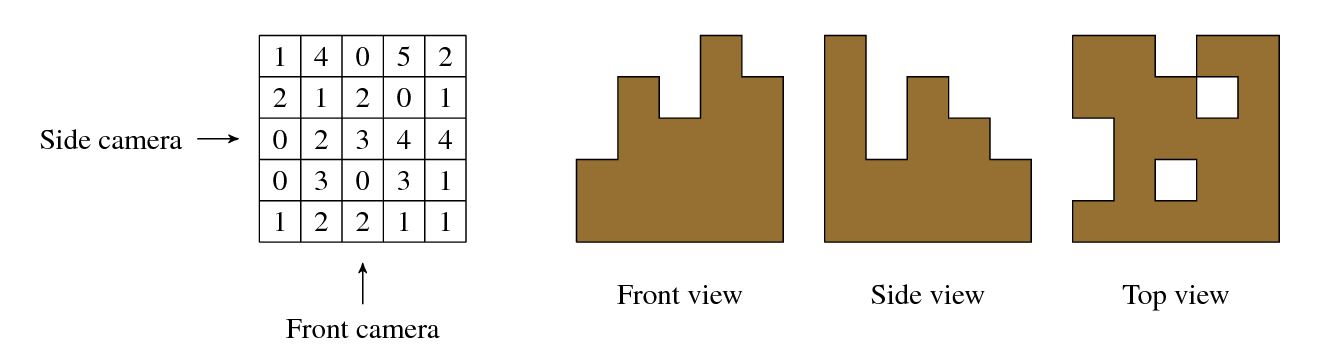
\includegraphics{mission_impossible_in.png}}
	\centerline{Une solution possible après un vol de 9 cartons~: 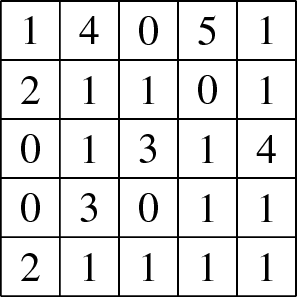
\includegraphics[width=2cm]{mission_impossible_out.png}}
\end{figure}

\source{Mission Improbable, ACM-ICPC World Finals 2017}
\source{aussi billet sur tryalgo.org du 31/05/2017}

\newpage 
\section{Champs boueux}

Vos vaches broutent dans un terrain qui se modélise comme une grille composée de $m$ lignes et de $n$ colonnes. Chaque case contient soit de l'herbe soit de la boue. Vous voulez couvrir toute la boue avec des planches rectangulaires. Ces planches ont la largeur de la case d'une grille, mais des longueurs arbitraires. Les planches ne doivent pas recouvrir de l'herbe.  Vous devez couvrir toute la boue avec un nombre minimum de planches pour cela, même si cela revient à couvrir plusieurs fois une même case. 


\begin{figure}[h]
	\centerline{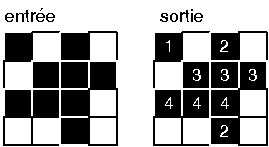
\includegraphics{boue.pdf}}
	Cette solution utilise 4 planches. Les planches 3 et 4 se superposent avec la planche 2.
\end{figure}

Réduisez ce problème vers un problème de couplage.

\source{Muddy Fields, SPOJ.com/problems/MUDDY}

\section{Flot maximum à coût minimum}

On vous donne un graphe $G(V,E)$, de nouveau avec deux sommets distincts $s,t\in V$ ainsi que des capacités sur les arêtes $c:E \rightarrow \mathbb N$ mais cette fois-ci également avec un coût sur les arêtes $w: E\rightarrow \mathbb N$.  L'interprétation est que chaque unité de flot traversant une arête $e$ génère un coût de $w(e)$ Euros.

Le but est de trouver un flot $f$ de $s$ à $t$ de valeur maximale, et qui minimise également le coût total $\sum_{e:f(e)>0} f(e) w(e)$.

Proposez un algorithme pour ce problème, en s'inspirant des algorithmes pour le cas sans coût.  Analysez sa complexité.
Indice~: vous pourriez par exemple chercher certains cycles dans le graphe.
\end{document}
